Once a PC surrogate has been constructed, it can be used in Bayesian inference on
model parameters and optimisation under uncertainty. The relevant mathematical techniques are
\begin{itemize}
\item Surrogate models in general.
\item Bayesian inference, with application to model parameters
\item Optimisation under uncertainty
\end{itemize}


\subsubsection{Surrogate Models}\label{sec:surrogate}

The current trend for forward UQ~(\Sec{forward}) in large-scale computational models, where the aim is to quantify 
the statistics of simulation outputs based on the assumed statistics of uncertain model parameters, 
has led to a need to perform large numbers of simulations in order to chart high-dimensional input 
parameter spaces (see, for example \cite{Su17Surr}).  
Brute-force application of Monte-Carlo using full accuracy {\it in-silico} models is 
impractical due to the requirement to perform possibly millions of simulations, if each
is required for one sample
since the convergence rate of MC scales as $\frac{1}{\sqrt{N}}$ for $N$~samples.
%(one might keep in mind the quote 
%from Edward Teller {\it `A state-of-the-art calculation requires 100 hours of CPU time on the 
%state-of-the-art computer, independent of the decade.'}).  
One solution is to view the simulation (regardless of its microscopic physics and myriad degrees of 
freedom) as a black box that takes input parameters and produces outputs, and then replace the full 
simulation by a {\it surrogate model} whose purpose is to reproduce the outputs of 
the simulator with an adequate degree of fidelity and at low cost.  
Surrogate models (also called response surfaces, metamodels, or emulators) must be calibrated using past 
knowledge of the simulator and by a limited number of full simulations for judiciously-chosen input 
parameter sets.
%(coverage of parameter space is key here, using techniques such as Latin cube 
%hypersampling and quasi-random numbers).

Modern methods for constructing surrogate models divide fairly neatly into regressions against sets 
of random variables, and machine learning based approaches.
A few examples of both types follow (further information can be found by following the links in 
\cite{SMwiki}).

\paragraph{Kriging} also known as \textbf{Gaussian process regression}, involves the assumption that the underlying uncertainty 
in the sample data follows a Gaussian process, that is, a stochastic process ${Z_x; x \in X}$ such 
that for every finite set of indices $x_1, ... , x_K$

\begin{equation}
Z_{x_1, ... , x_K} = \left ( Z_{x_1}, ... Z_{x_K} \right )
\end{equation}

is a multivariate Gaussian variable.  An equivalent (characteristic function) definition is the
statement that there exist 
real-valued $\sigma_{jk}$, $\mu_j$ for any $s_1, ... , s_K \in \mathbb{R}$ such that the 
expectation is

\begin{equation}
\mathbb{E} \left ( \exp \left ( i \sum_{k=1}^K {s_k Z_{x_k} }\right ) \right ) = \exp \left ( 
-\frac{1}{2} \sum_{j,k} \sigma_{jk} s_j s_k + i \sum_{j}{\mu_j s_j } \right ).
\end{equation}

The $\mu_j$ are the means of the process and the $\sigma_{jk}=C(x_i, x_j)$ the covariances.  
The latter are typically chosen from a standard dictionary of functions.
%(hyperparameters of the candidate model typically being derived using Bayesian methods)
Common choices correspond to 
well-known stochastic processes and include Gaussian white noise,

\begin{equation}\label{eq:stoch}
C(x_i, x_j) = \sigma^2 \delta(x_i-x_j);
\end{equation}

Ornstein-Uhlenbeck, which is used to describe the velocity of a particle under the influences of 
damping and Brownian motion,

\begin{equation}\label{eq:OU}
C(x_i, x_j) = \exp \left ( -\frac{|x_i-x_j|}{L}\right );
\end{equation}

and Mat\'ern, 

\begin{equation}\label{eq:matern}
C(x_i, x_j) = \sigma^2 \frac{2^{1-\nu}}{\Gamma(\nu)} \left ( \sqrt{2 \nu} \frac{x_i-x_j}{L} \right 
)^{\nu} K_{\nu} \left ( \sqrt{2 \nu} \frac{x_i-x_j}{L} \right)
\end{equation}

which has a number of desirable properties, for example the ability to model a process that is 
discontinuous at a chosen order of derivative ($K_{\nu}$ is the modified Bessel function of the 
second kind). In the above \Eqs{stoch}{matern}, $\sigma$, $L$ and $\nu$ are examples of
hyperparameters, which are typically determined by use of Bayesian methods.

In {\it simple kriging} the mean $\mu$ is known in advance and the estimator for the value of the 
process at point $x$ is constructed as a weighted linear combination of the existing set of $N$ 
samples

\begin{equation}
\tilde{Z}(x) = \mu + \sum_{i=1}^N w_i \left ( Z(x_i) - \mu \right );
\end{equation}

minimisation of the prediction variance leads to a simple expression (actually a least-squares 
estimator) for the weights in terms of the matrix of covariances between the sample points $C_{ij} 
\equiv C(x_i,x_j)$ and the vector of covariances between the estimation point and the sample points 
$r_i \equiv C(x, x_i)$ as ${\mathbf w} =  {\bf r} C^{-1}$.

In the case of a constant unknown mean, one has {\it ordinary kriging} (note it still involves the 
assumption that the mean is constant), and the formulae above are supplemented by a condition that 
the estimator be unbiased (this is simply the constraint that the weights sum to unity), which can 
be incorporated using a Lagrange multiplier.  
There are successively more involved kriging varieties based on further generalisation, for example 
general polynomial models of the underlying trend.  
The variance of the estimator can be computed, leading to an intuitive plot that resembles a string 
of sausages (\Fig{kriging}) in the more general case.  
Note that there is also gradient-enhanced kriging, which uses an estimate of the local gradient to 
reduce the variance of a kriging estimator.

\begin{figure}
\centerline{\rotatebox{0}{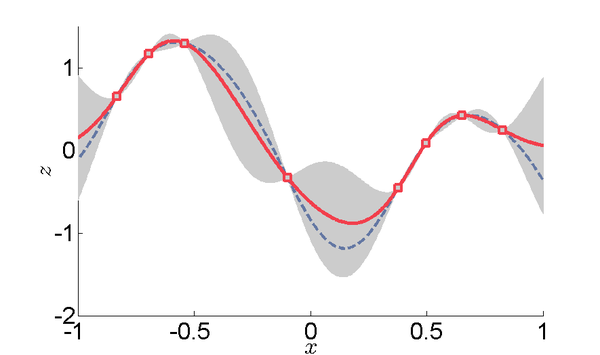
\includegraphics[width=10.5cm]{../png/kriging.png}}}
\caption{\label{fig:kriging}
Kriging estimator (red curve) and its associated standard deviation (grey).  
The dotted line shows a plausible spline fit that nevertheless departs from the Maximum 
Likelihood kriging fit.  Taken from \cite{krigingwiki}.}
\end{figure}

\paragraph{Generalised Polynomial Chaos~(gPC)} involves expanding model outputs $Y$ in terms of orthogonal polynomials of 
random variable inputs $X$ (orthonormality being defined with respect to the measure associated to 
the distribution of the $X$ - e.g. Hermite polynomials in the normal-distributed case).  
Construction of the surrogate is then reduced to the task of determining the coefficients in the expansion 
(which obviously is truncated at some polynomial order); this can be accomplished by means of 
least-squares analysis.  
Once the coefficients are available, the truncated PCE can be sampled at negligible cost and thus 
the full probability density function of the output is available, as is access to the sensitivity analysis via Sobol indices 
which represent the portion of the output variance due to each input parameter or combination of 
parameters (see \Sec{stage1} for more details).  

\paragraph{Artificial Neural Networks~(ANNs)} are models consisting of arrays of 
interconnected nodes (artificial neurons) that react to inputs in a non-linear way.  
The neurons (nodes) and connecting edges have {\it weights} associated to them that control the 
output for a given set of inputs: these weights are dynamically adjusted in response to training 
feedback taking the form of an error measure, a process called {\it unsupervised learning}.  
Such general models abandon any attempt to match the model to the specific problem, with 
specificity emerging as a result of what is usually extensive training.

The input to a typical neural network is a vector of elements ${x_k}$, which are combined by a 
series of linear filters to give inputs to the {\it hidden unit} neurons
\begin{equation}
h_j = \sum_k w_{jk} x_k,
\end{equation}
the output of which is a function of the input
\begin{equation}
X_j = g(h_j),
\end{equation}
where the {\it activation functions} $g$ are nonlinear.  
Typically chosen to suppress large outputs, they are frequently sigmoid in form; one such choice is 
$\tanh(\beta h)$.  
The topology of the network often corresponds to a number of `layers' followed by a final set of 
output nodes, see \cite{gershenfeld}, \cite[\S\,6.7]{bruntonkutz}.

Such a generality of models provides potential surrogates for a wide range of problems 
including situations where the model exhibits discontinuities in its derivatives.
The selection of an appropriate member of the {\it neural network zoo}~\cite{asimovwebsite} is
a further challenge. Both the `zoo' and ref~\cite[\S\,6.7]{bruntonkutz} give brief indications
as to which ANN topologies might be most appropriate. Within a given topology, it of
course desirable to identify the number of minimum number of neurons needed, although this
is probably less critical in application to \nep.
%Often, most of the work lies in the offline training stage (though in complex cases this process 
%can be very costly), giving an affordable online surrogate.

%\paragraph{Support Vector Machines~(SVMs)} are a class of supervised learning models that use learning 
%algorithms based on classification: given a set of training examples, a SVM is able to classify a 
%given object according to a non-probabilistic binary linear classifier.  
%The simplest example is the problem of determining the $p$-dimensional hyperplane dividing two sets 
%of samples $a$ and $b$, given that those sets are linearly separable, and choosing the hyperplane 
%such that the minimum distance from the hyperplane to any item of data is maximized (note that 
%these closest data points are referred to as the support vectors).  
%This {\it maximum-margin} hyperplane is chosen by noting that the two parallel hyperplanes given by
%
%\begin{eqnarray}
%{\mathbf w} \cdot {\mathbf x} - b &=& 1\\
%{\mathbf w} \cdot {\mathbf x} - b &=& -1
%\end{eqnarray}
%
%are separated by the Euclidean distance $\x=2/\lVert {\mathbf w} \rVert$, and so the problem is 
%to minimize $\lVert {\mathbf w} \rVert$ subject to the constraint that $y_i({\mathbf w} \cdot {\mathbf x_i}-b) 
%\geq 1$ (in the simple case that the two data sets correspond respectively to values $1$ and $-1$) 
%- this is the criterion that no data points lie within the margin.  
%The linear classifier is then the sign of ${\mathbf w} \cdot {\mathbf x} - b$ (see \Fig{svm} for an 
%illustration of this).  
%In general, the sample set may not be linearly separable and a way to get round this is to replace 
%the scalar product with a nonlinear {\it kernel function}, which basically allows the boundary 
%between sets to be a curve.  
%Such generalisations have the appealing feature that the solution is obtained via a convex 
%optimisation problem, see ref~\cite{svmwiki}.
%
%\begin{figure}
%\centerline{\rotatebox{0}{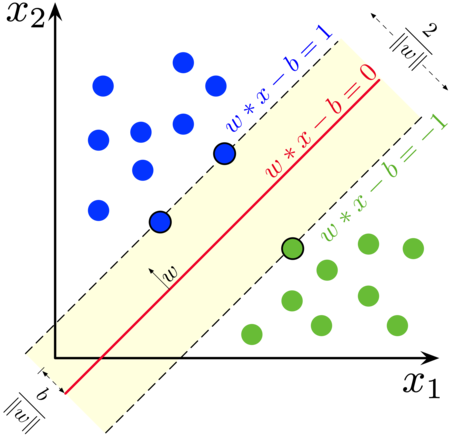
\includegraphics[width=7.5cm]{../png/svm_margin.png}}}
%\caption{\label{fig:svm}
%Illustration of the construction of a binary linear classifier for a linearly separable data set,  
%taken from \cite{svmwiki}.}
%\end{figure}

\paragraph{Reduced-order models~(ROMs)} are commonly produced using projection methods in which the dynamics of the
full forward problem are projected onto a reduced-dimensional subspace.  
The latter is generally assembled using proper orthogonal decomposition or reduced basis methods, 
and using a set of full simulation outputs (`snapshots').  
The success of these methods is connected with the merits of `diagonalising' the problem to a set 
of uncorrelated degrees of freedom and identifying the components that have the biggest 
eigenvalues, a procedure known generically as principal components analysis.  
As with the methods outlined above, the reward is a more parsimonious way of calculating the model 
dynamics, see \cite{MORwiki}. These models will be discussed in more detail as part of the
Milestone Report~M2.5.2 scheduled for August~2021.

\subsubsection{Bayesian Inference as Applied to Model Parameters}\label{sec:Bayes}

The general problem of modeling a physical system involves the need to fit a model of some kind to 
existing data: there is a model architecture, $m$, with a set of adjustable parameters $\theta$, 
as well as some measured data $\x$, and the goal is to choose (or, in statistics jargon, {\it 
infer}) $\theta$ so as to provide the best agreement to $\x$.
This is also referred to as ``Inverse UQ", to be contrasted with 
``Forward UQ"  where the input distributions are given 
and the aim is to estimate the the uncertainties in the outputs.

The Bayesian formulation of this inverse problem relies on evaluating the $\theta$ that are most 
likely, given the model, the measured data, and, crucially, our prior beliefs about what parameters 
are plausible - leading to {\it conditional probability}.  
The fundamental tool for performing this sort of `turnaround' of conditional probabilities is {\it 
Bayes' rule}, which gives us the following quantity to maximise, called the {\it posterior 
distribution}:

\begin{equation}
\mathrm{max} \left ( p (\theta | \x,m) \right ) = \mathrm{max} \left ( 
\frac{p(\x|\theta,m)p(\theta|m) }{p(\x|m) = \int p(\x|\theta,m) p(\theta|m) \x d\theta} \right ),
\end{equation} 

the right-hand side of which (whose term $p(\x|\theta,m)$ represents the probability of having 
obtained the data $\x$ given parameters $\theta$ and model $m$; $p(\theta|m)$ represents advance 
belief about which values of the parameters are reasonable - the Bayesian {\it prior}; the 
denominator being essentially a normalising factor) can be expressed illustratively as

\begin{equation}
\mathrm{max} \left ( \frac{likelihood \times prior }{evidence} \right ).
\end{equation}

A full Bayesian model such as this involves, potentially, a great amount of work.  
Not only must a high-dimensional normalisation integration be performed, but there are {\it two} 
optimisation loops, one over the set of parameters, and also a maximisation over possible model 
architectures as well.  To reduce the workload, the decision might be taken to use only one model architecture, 
leading to the problem

\begin{equation}
\mathrm{max} \left ( p(\theta|\x) \right ) = \mathrm{max} \left ( \frac{p(\x|\theta)p(\theta) 
}{p(\x)} \right ).
\end{equation}

This is called {\it Maximum A Posteriori} (MAP) estimation (note that it uses the {\it modal} value 
- the maximum of the distribution).  
An additional simplification is to note that the normalisation integral in the denominator can be 
disregarded as it does not affect the position of the maximum.

Further assuming a uniform prior leads to the simplest kind of model estimation, {\it Maximum 
Likelihood} (which one might also say is not really Bayesian at all):

\begin{equation}
\mathrm{max} \left ( p(\theta|\x) \right ) = \mathrm{max} \left ( p(\x| \theta) \right ).
\end{equation}

Maximum Likelihood leads to the familiar and much-used least-squares error measure, which is the 
Maximum Likelihood estimator for data with normally distributed errors (another detail is that the 
sums of squared normal variables obey the chi-squared distribution ubiquitous in elementary 
goodness-of-fit testing).  
Model fitting using least-squares is achieved by using the matrix pseudo-inverse $\left ( 
M^{\dagger} M \right)^{-1} M^{\dagger}$ to derive (few) model parameters from (many) data points, 
actually a case of singular value decomposition (SVD).  
There are other worthwhile tricks e.g. writing strictly positive parameters as the square of 
something else before fitting (this can be used to avoid getting e.g. negative fitted variance 
hyperparameters).  For more details, see, for example, \cite{gershenfeld}.

\subsubsection{Optimisation Under Uncertainty~(OUU)}\label{sec:OUU}

The problem of Optimisation Under Uncertainty~(OUU) is an expanding area in the wider field of
Operational Research, and also in 
engineering where it may be the case that simple deterministic optimisations turn out not to be
sufficiently robust when say devices are built with the tolerances typical of many construction methods.
%real-world fabrication methods.  
%Basic extensions involve the evaluation of gradients and Hessians in the vicinity of such 
%non-aleatoric optima.  
%Another approach is that of {\it robust optimisation}, in which a certain measure of robustness is 
%sought against a deterministic variability in the input parameters (i.e. a tolerance).  One popular 
%measure of local robustness is the {\it radius of stability} model, in which the set of acceptable 
%outcomes is quantified by the radius of the largest ball in parameter space for which certain 
%performance or stability requirements are realized.
%However, these approaches offer purely local information; for a global perspective, a stochastic 
%analysis is needed, enabling the incorporation of valuable prior information about the distribution 
%of model inputs.
Obtaining solutions which provide the optimal value for a given `objective function'
normally involves many simulation runs, which now have to cover
the set of parameters characterising uncertainty, thereby
{\it `inheriting and magnifying all the difficulties of forward UQ'}~(\cite{Na18Unce}).
It is clear that this motivates the use of lower fidelity and surrogate models to the fullest practical extent.
 


%In addition, explorations of parameter space often need to navigate regions where either codes or 
%models (or both) fail.  
Najm and coworkers~\cite{Ge19Prog} have integrated the well-known DAKOTA package for UQ~\cite{dakota6,dakotawebsite}
with the package SNOWPAC (Stochastic Nonlinear Optimisation 
with Path-Augmented Constraints) to perform OUU, see the example in \Fig{ouuworkflow}.
The workflow begins on the left, with an offline model reduction using global sensitivity
analysis (GSA), compressed sensing techniques 
(CS) applied to polynomial chaos expansions (PCE) and multi-level Monte-Carlo (MLMC)
as described in the preceding \Sec{stage1}~and~\Sec{stage2}. 
The inclusion of uncertainty means that the objective function and the constraints have to become functions of the parameters~$\theta_i$.
In ref~\cite{Ge19Prog} the objective function is eg.\ taken to be a robustness measure given by a linear combination of the 
expectation value and the standard deviation i.e. $\mathbb{E}(Q) + c \mathrm{Var}[Q]$,
for some constant $c>0$.  
The optimisation driven by the DAKOTA plus SNOWPAC combination, incorporates forward uncertainty quantification using MLMC or 
adaptive sparse quadrature multi-level multi-fidelity (ASQ-MLMF) modeling.  Note the `simulator' 
used during the optimisation is likely to be a surrogate model.
%DAKOTA provides a flexible interface for optimisations using 
%different sampling strategies and surrogate models, and incorporates a Multi-level Monte-Carlo 
%estimator as described in \Sec{mlmc}.

%The DAKOTA toolkit is written in C++ and it {\it `... provides a flexible, extensible interface 
%between simulation codes and a variety of iterative systems analysis methods, including 
%optimisation, uncertainty quantification, deterministic/stochastic calibration, and 
%parametric/sensitivity/variance analysis'} \cite{dakotawebsite}.  
%The software is maintained by Sandia National Laboratories and is open-source under GNU LGPL.

\begin{figure}
\centerline{\rotatebox{0}{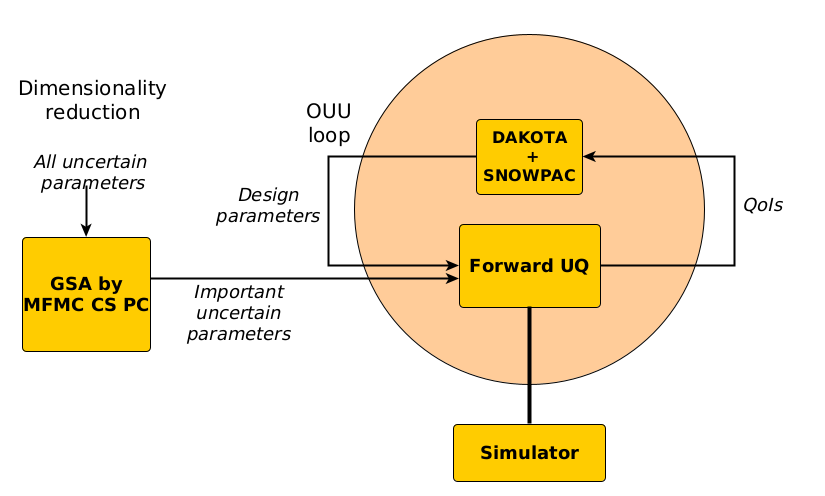
\includegraphics[width=13.5cm]{../png/OUUWA.png}}}
\caption{\label{fig:ouuworkflow}
Workflow for optimisation under uncertainty (after \cite{Na18Unce}).}
\end{figure}

%The MLMC estimator of the expectation value of $Q_L$  - the QoI evaluated at the finest resolution 
%level - and its variance can be expanded as
%
%\begin{eqnarray}
%\mathbb{E}(Q_L) \approx \hat{Q}^{ML}_L &=& \sum_{l=0}^L \frac{1}{N_l} \sum_{i=1}^{N_l} \left ( 
%Q_l^{(i)}-Q_{l-1}^{i} \right ) = \sum_{l=0}^L \hat{Y}_l\\
%\mathrm{Var}[\hat{Q}^{ML}_L] &=& \sum_{l=0}^L \frac{1}{N_l} \mathrm{Var}[Y_l].
%\end{eqnarray}
%
%Here $Y_l$ is the difference function between two successive levels and $\hat{Y}_l$ its estimator 
%at the $l$th level.  
%The utility of the MLMC is that, if it is reasonable to assume that $\mathrm{Var}[Y_L] \rightarrow 
%0$ as $l \rightarrow 0$, then the number of samples $N_l$ at each level decreases for increasing 
%$l$.  
%The standard error in the mean can be obtained as the square root of $\mathrm{Var}[\hat{Q}_L^{ML}]$ 
%because the distribution of the MLMC estimator approaches a Gaussian for a large sample size; the 
%standard error in the standard deviation is not available in closed form and its calculation 
%involves approximation.  
